
%(BEGIN_QUESTION)
% Copyright 2013, Tony R. Kuphaldt, released under the Creative Commons Attribution License (v 1.0)
% This means you may do almost anything with this work of mine, so long as you give me proper credit

Write an equation describing the output voltage as a function of temperature, assuming the RTD (Resistive Temperature Detector) has a resistance predicted by the following formula, where $T$ is in degrees Celsius:

$$R_{RTD} = 100 (1 + 0.00385T)$$

$$\includegraphics[width=15.5cm]{i03546x01.eps}$$

\vskip 30pt

$V_{out} = f(T) = $

\vskip 30pt

Next, calculate the RTD temperature at a measured output voltage of 3.5 volts.

\underbar{file i03546}
%(END_QUESTION)





%(BEGIN_ANSWER)

$$V_{out} = 6 \left(150 \over 250 + 0.385T \right)$$

\vskip 10pt

$T$ = 18.55 $^{o}$C when $V_{out}$ = 3.5 volts.

%(END_ANSWER)





%(BEGIN_NOTES)

{\bf This question is intended for exams only and not worksheets!}.

%(END_NOTES)


